% Fig. 3: error of the front positions versus grid step.
% Data: ../code/out/fig3_errors.dat (produced by ../code/make_fig3_data.py).
% Compile with pdflatex, then  pdftops -eps Fig3_convergence.pdf Fig3.eps
\documentclass[border=2pt]{standalone}
\usepackage{pgfplots}
\pgfplotsset{compat=1.18}
\begin{document}
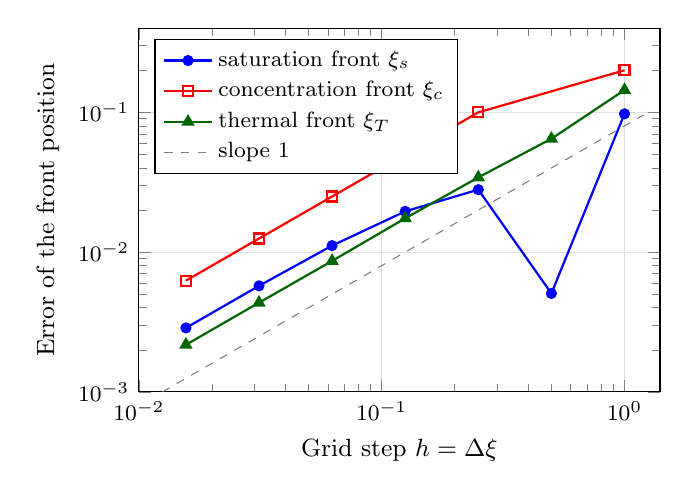
\begin{tikzpicture}
\begin{loglogaxis}[
  width=8.2cm, height=6.2cm,
  xlabel={Grid step $h=\Delta\xi$},
  ylabel={Error of the front position},
  xmin=0.01, xmax=1.4, ymin=1e-3, ymax=0.4,
  grid=major, grid style={gray!25},
  legend pos=north west, legend style={font=\footnotesize, cells={anchor=west}},
  tick label style={font=\footnotesize}, label style={font=\small},
]
% saturation front xi_s
\addplot[blue, thick, mark=*, mark size=1.6pt] coordinates {
  (1.000000,9.762079e-02) (0.500000,5.060730e-03) (0.250000,2.799679e-02)
  (0.125000,1.957145e-02) (0.062500,1.113290e-02) (0.031250,5.736882e-03)
  (0.015625,2.868441e-03)};
\addlegendentry{saturation front $\xi_s$}
% concentration front xi_c (zero error for h = 1/2 is not shown)
\addplot[red, thick, mark=square, mark size=1.8pt] coordinates {
  (1.000000,2.000000e-01)
  (0.250000,1.000000e-01) (0.125000,5.000000e-02) (0.062500,2.500000e-02)
  (0.031250,1.250000e-02) (0.015625,6.250000e-03)};
\addlegendentry{concentration front $\xi_c$}
% thermal front xi_T
\addplot[black!60!green, thick, mark=triangle*, mark size=2pt] coordinates {
  (1.000000,1.444777e-01) (0.500000,6.475508e-02) (0.250000,3.424385e-02)
  (0.125000,1.745300e-02) (0.062500,8.647505e-03) (0.031250,4.346842e-03)
  (0.015625,2.173421e-03)};
\addlegendentry{thermal front $\xi_T$}
% reference slope 1
\addplot[gray, dashed, domain=0.0125:1.2, samples=2] {0.08*x};
\addlegendentry{slope 1}
\end{loglogaxis}
\end{tikzpicture}
\end{document}
